\documentclass[11pt,a4paper]{ltjsarticle}
\usepackage{luatexja}
\usepackage{luatexja-fontspec}
\usepackage{amsmath,amssymb}
\usepackage{geometry}
\geometry{left=2.5cm,right=2.5cm,top=3cm,bottom=3cm}
\usepackage{graphicx}
\usepackage{booktabs}
\usepackage{siunitx}
\sisetup{detect-all,detect-weight=true,detect-family=true, per-mode=symbol}
% decadeとdBの単位を定義
\DeclareSIUnit\decade{decade}
\DeclareSIUnit\dB{dB}
\usepackage{hyperref}
\usepackage{url}
\usepackage{fancyhdr}
\usepackage{fontspec}
\usepackage{unicode-math}
\usepackage{pgfplots}
\pgfplotsset{compat=1.18}

% 欧文フォント設定
\setmainfont{Times New Roman}
\setsansfont{Arial}
\setmonofont{Consolas}

% 日本語フォント設定
\setmainjfont{Yu Mincho}
\setsansjfont{Yu Gothic}

% 数式フォント設定
\setmathfont{XITS Math}

% 参考文献番号を右肩に上付き表示するためのカスタムコマンド
\newcommand{\supcite}[1]{\textsuperscript{\cite{#1}}}

% ヘッダー設定
\pagestyle{fancy}
\fancyhead{}
\fancyhead[R]{\footnotesize
  ボード線図の解析による伝達関数の導出 \\
  長野高専 電気電子工学科 5年 34番 栁原魁人 \\
  \today
}
\setlength{\headheight}{34.832pt}

\begin{document}

\title{ボード線図の解析による伝達関数の導出}
\author{長野高専 電気電子工学科 5年 34番 氏名 栁原魁人}
\date{\today}
\maketitle
\thispagestyle{fancy}

\section{問1の解析(一次遅れ系)}

\subsection{ボード線図の初期分析とシステムの同定}

提供されたゲイン線図1を分析し,このシステムが一次遅れ系としてモデル化できることを確認する.

\begin{itemize}
    \item \textbf{周波数応答の観察:} グラフの横軸は対数スケールの周波数(\si{\hertz}),縦軸はゲイン(\si{\decibel})を示している\supcite{ref1}.
    \item \textbf{低周波域の特性:} \SI{0.1}{\hertz}のような低い周波数では,ゲインは約\SI{+5}{\decibel}で一定である\supcite{ref1}.この平坦な領域は,システムの直流ゲイン(定常ゲイン)を示している.
    \item \textbf{高周波域の特性:} ある周波数(コーナー周波数)を超えると,ゲインは対数グラフ上で直線的に減少し始める.この傾きを確認すると,一次遅れ系の特徴と一致することがわかる.例えば,\SI{1}{\hertz}(ゲイン約\SI{2}{\decibel})から\SI{10}{\hertz}(ゲイン約\SI{-15}{\decibel})までの1ディケード(周波数が10倍)の区間で,ゲインは約\SI{17}{\decibel}減少している.これは,一次遅れ系の理論的な減衰傾度である\SI{-20}{\dB\per\decade}に非常に近い値である\supcite{ref2}.
\end{itemize}

この\SI{-20}{\dB\per\decade}という傾きは,システムの高周波応答が単一のエネルギー蓄積要素(数学的には単一の極)によって支配されていることを示す決定的な特徴である.入力信号の周波数が10倍になるごとに出力信号の振幅が10分の1($10^{-20/20} = 0.1$倍)に減衰することを意味する.このグラフの特性から,問題の仮定通り,このシステムを一次遅れ系として扱うことの妥当性が確認できる.

\subsection{システムパラメータの段階的導出}

一次遅れ系の伝達関数 $G_1(s) = \frac{K}{Ts+1}$ を決定するために必要なパラメータ,すなわち直流ゲイン $K$ と時定数 $T$ を順に求める.

\subsubsection{直流ゲイン $K$ の計算}

直流ゲインは,周波数がゼロに近い低周波域におけるシステムのゲインである.グラフの低周波域の漸近線から,ゲイン $G_{\text{dB}}$ は\SI{5}{\decibel}と読み取れる\supcite{ref1}.

ゲインのデシベル値 $G_{\text{dB}}$ と真数(リニアスケール)のゲイン $K$ の関係は $G_{\text{dB}} = 20\log_{10}(K)$ で与えられる\supcite{ref4}.この式を用いて $K$ を計算する.
\begin{enumerate}
    \item $5 = 20\log_{10}(K)$
    \item $\log_{10}(K) = \frac{5}{20} = 0.25$
    \item $K = 10^{0.25} \approx 1.778$
\end{enumerate}
この値 $K$ は,非常にゆっくりとした定常的な入力信号に対する出力信号の振幅比を表す.

\subsubsection{コーナー周波数 \texorpdfstring{$f_c$}{fc} の決定}

コーナー周波数を決定するには,2つの主要な方法がある.両方を用いることで,実験データからより正確な値を推定できる.問題の指示である「図に補助線を入れる」というのは,特に漸近線近似法を指している\supcite{ref1}.

\paragraph{方法A:漸近線近似法(作図による方法)}
\begin{enumerate}
    \item \textbf{低周波漸近線の作図:} 直流ゲインである\SI{+5}{\decibel}の高さに水平な直線を引く.
    \item \textbf{高周波漸近線の作図:} ゲインが減少している部分に最もよく沿うように,\SI{-20}{\dB\per\decade}の傾きを持つ直線を引く.この直線は,例えば\SI{10}{\hertz}において約\SI{-15}{\decibel}の点を通過する.
    \item \textbf{交点の特定:} これら2本の漸近線が交差する点の周波数がコーナー周波数 $f_c$ となる.図上でこれらの補助線を描くと,交点は約 $f_c = \SI{1.0}{\hertz}$ となる.
\end{enumerate}

\paragraph{方法B:-3 dB法(検証)}
コーナー周波数は,ゲインが直流ゲインから正確に\SI{3}{\decibel}低下した点の周波数としても定義される\supcite{ref4}.
\begin{enumerate}
    \item 目標ゲインの計算: 目標となるゲインは,直流ゲインから\SI{3}{\decibel}を引いた値である.
    目標ゲイン = \SI{5}{\decibel} - \SI{3}{\decibel} = \SI{2}{\decibel}
    \item \textbf{グラフ上での周波数の特定:} グラフ上でゲインが\SI{2}{\decibel}となる周波数を探す.プロットを詳細に確認すると,ゲイン曲線が\SI{2}{\decibel}のレベルを通過するのは,約 $f_c = \SI{1.0}{\hertz}$ であることがわかる\supcite{ref1}.
\end{enumerate}
両方の方法で一致した結果が得られたため,コーナー周波数は\SI{1.0}{\hertz}であると結論付けられる.

\subsubsection{角周波数 \texorpdfstring{$\omega_c$}{ωc} への変換と時定数 \texorpdfstring{$T$}{T} の計算}

伝達関数では通常,周波数 $f$ (\si{\hertz}) ではなく角周波数 $\omega$ (\si{\radian\per\second}) を用いる.変換式は $\omega = 2\pi f$ である.
\begin{itemize}
    \item コーナー角周波数 $\omega_c = 2\pi \times f_c = 2\pi \times 1.0 \approx \SI{6.283}{\radian\per\second}$
\end{itemize}
一次遅れ系において,時定数 $T$ はコーナー角周波数の逆数で与えられる ($T=1/\omega_c$)\supcite{ref2}.
\begin{itemize}
    \item 時定数 $T = \frac{1}{\omega_c} = \frac{1}{6.283} \approx \SI{0.159}{\second}$
\end{itemize}
この時定数 $T$ は,システムのステップ応答が最終値の約63.2\%に達するまでにかかる時間を表し,周波数領域の特性と時間領域の挙動を結びつけます\supcite{ref5}.

\subsection{最終的な伝達関数 \texorpdfstring{$G_1(s)$}{G1(s)} の定式化}

算出したパラメータ $K$ と $T$ を一次遅れ系の標準的な伝達関数の形式に代入する.
\begin{itemize}
    \item \textbf{標準形式:} $G_1(s) = \frac{K}{Ts+1}$
    \item \textbf{値の代入:}
    $G_1(s) = \frac{1.778}{0.159s+1}$
\end{itemize}
この式が,問1のボード線図で示されたシステムの動特性を表す伝達関数である.

\begin{table}[htbp]
  \centering
  \caption{一次遅れ系のパラメータ導出概要}
  \label{tbl:param1}
  \begin{tabular}{@{}lllc@{}}
    \toprule
    パラメータ & 記号 & グラフからの読み取り / 計算 & 最終値 \\
    \midrule
    直流ゲイン (\si{\decibel}) & $G_{\text{dB}}$ & \SI{5}{\decibel} & - \\
    直流ゲイン (真数) & $K$ & $10^{(5/20)}$ & 1.778 \\
    コーナー周波数 (\si{\hertz}) & $f_c$ & \SI{1.0}{\hertz} & - \\
    コーナー周波数 (\si{\radian\per\second}) & $\omega_c$ & $2\pi \times 1.0$ & \SI{6.283}{\radian\per\second} \\
    時定数 & $T$ & $1/\omega_c$ & \SI{0.159}{\second} \\
    \bottomrule
  \end{tabular}
\end{table}

\section{問2の解析(二次遅れ系)}

\subsection{ボード線図の初期分析とシステムの同定}

問2で提供されたゲイン線図と位相線図を分析し,減衰の小さい(不足減衰)二次遅れ系の特徴を確認する\supcite{ref1}.

\begin{itemize}
    \item \textbf{軸の確認:} 横軸は対数スケールの角周波数 (\si{\radian\per\second}),縦軸はゲイン (\si{\decibel}) と位相 (\si{\degree}) です\supcite{ref1}.
    \item \textbf{直流ゲイン:} 低周波域において,ゲイン線図は\SI{0}{\decibel}で平坦になっている\supcite{ref1}.
    \item \textbf{共振ピーク:} ゲイン線図には顕著なピーク(とがり)が見られる.これは,減衰の小さい二次遅れ系が示す共振現象の典型的な特徴である\supcite{ref3}.グラフ上のデータチップにより,このピークの座標が\textbf{角周波数 \SI{54.5}{\radian\per\second}} で \textbf{最大ゲイン \SI{4.84}{\decibel}} であることが明示されている\supcite{ref1}.
    \item \textbf{高周波域の減衰:} ピークを過ぎた高周波域では,ゲインの減衰傾度は一次遅れ系よりも急峻である.これは,二次遅れ系の理論的な傾きである\SI{-40}{\dB\per\decade}と一致する\supcite{ref3}.
    \item \textbf{位相変化:} 位相線図を見ると,位相遅れが低周波域の\SI{0}{\degree}から始まり,共振周波数付近で\SI{-90}{\degree}を通過し,高周波域で\SI{-180}{\degree}に漸近している\supcite{ref7}.この\SI{180}{\degree}にわたる位相変化は,システムが2つの極を持つ二次系の特徴である.
\end{itemize}

二次遅れ系のパラメータ($K$, $\zeta$, $\omega_n$)は相互に密接に関連している.共振ピークの高さ ($M_p$) は主に減衰係数 $\zeta$ によって決まり,共振ピーク周波数 ($\omega_r$) は固有角周波数 $\omega_n$ と減衰係数 $\zeta$ の両方に依存する.このため,パラメータを導出するには特定の順序で計算を進める必要がある.まず直流ゲインから $K$ を求め,次にピークの高さから $\zeta$ を計算し,最後にピーク周波数と求めた $\zeta$ を用いて $\omega_n$ を算出するという手順が最も合理的である.

\subsection{システムパラメータの段階的導出}

上記の戦略に従い,二次遅れ系の標準伝達関数 $G_2(s) = \frac{K\omega_n^2}{s^2 + 2\zeta\omega_n s + \omega_n^2}$ のパラメータ $K$, $\zeta$, $\omega_n$ を決定する\supcite{ref8}.

\subsubsection{直流ゲイン $K$ の計算}

グラフの低周波漸近線から,ゲインは\SI{0}{\decibel}です\supcite{ref1}.これを真数ゲイン $K$ に変換する.
\begin{itemize}
    \item $K = 10^{(G_{\text{dB}}/20)} = 10^{(0/20)} = 10^0 = 1$
\end{itemize}
このシステムは,直流(定常)入力に対しては入出力比が1となる.

\subsubsection{共振ピークゲイン \texorpdfstring{$M_{p,\text{dB}}$}{Mp,dB} と共振角周波数 \texorpdfstring{$\omega_r$}{ωr} の読み取り}

これらの値はグラフ上のデータチップによって直接与えられている\supcite{ref1}.
\begin{itemize}
    \item 共振ピークゲイン: $M_{p,\text{dB}} = \SI{4.84}{\decibel}$
    \item 共振角周波数: $\omega_r = \SI{54.5}{\radian\per\second}$
\end{itemize}

\subsubsection{減衰係数 \texorpdfstring{$\zeta$}{ζ} の計算}

減衰係数 $\zeta$ は,共振ピークの高さから計算できる.
\begin{enumerate}
    \item ピークゲインの真数値への変換: 減衰係数を求める公式は真数(リニアスケール)のゲイン $M_p$ を用いるため,まずdB値を変換する.
    $M_p = 10^{(M_{p,\text{dB}}/20)} = 10^{(4.84/20)} = 10^{0.242} \approx 1.746$
    \item 共振ピークの公式の適用: 不足減衰系 ($\zeta < 1$) における真数のピークゲイン $M_p$ と減衰係数 $\zeta$ の関係は,次式で与えられる.
    $M_p = \frac{1}{2\zeta\sqrt{1-\zeta^2}}$
    共振ピークが存在することから,$\zeta < 1/\sqrt{2} \approx 0.707$ であることがわかる\supcite{ref3}.
    \item \textbf{$\zeta$ の求解:} 上式に $M_p$ の値を代入し,$\zeta$ について解く.
    \begin{itemize}
        \item $1.746 = \frac{1}{2\zeta\sqrt{1-\zeta^2}}$
        \item $2\zeta\sqrt{1-\zeta^2} = \frac{1}{1.746} \approx 0.5727$
        \item 両辺を2乗する: $(2\zeta\sqrt{1-\zeta^2})^2 = 0.5727^2$
        \item $4\zeta^2(1-\zeta^2) = 0.3280$
        \item $4\zeta^2 - 4\zeta^4 = 0.3280$
        \item 整理して,$\zeta^4$ の項を正にする: $4\zeta^4 - 4\zeta^2 + 0.3280 = 0$
        \item これは $\zeta^2$ に関する二次方程式である.$x=\zeta^2$ とおくと,$4x^2 - 4x + 0.3280 = 0$ となる.解の公式を用いて $x$ を求める.
        \item $x = \frac{-(-4) \pm \sqrt{(-4)^2 - 4(4)(0.3280)}}{2(4)} = \frac{4 \pm \sqrt{16 - 5.248}}{8} = \frac{4 \pm \sqrt{10.752}}{8} = \frac{4 \pm 3.279}{8}$
        \item これにより,$x=\zeta^2$ の解として,$x_1 = \frac{7.279}{8} \approx 0.91$ と $x_2 = \frac{0.721}{8} \approx 0.090$ の2つが得られる.
        \item 前述の通り,共振が生じるのは $\zeta < 1/\sqrt{2}$,すなわち $\zeta^2 < 0.5$ の場合である.したがって,物理的に意味のある解は小さい方の $x_2$ である.
        \item $\zeta^2 = 0.090 \implies \zeta = \sqrt{0.090} \approx 0.30$
    \end{itemize}
\end{enumerate}
減衰係数は約 $\zeta=0.30$ と求められる.

\subsubsection{固有角周波数 \texorpdfstring{$\omega_n$}{ωn} の計算}

次に,共振角周波数 $\omega_r$ と減衰係数 $\zeta$ を用いて,システムの固有角周波数 $\omega_n$ を計算する.
\begin{enumerate}
    \item 共振角周波数の公式の適用: 固有角周波数 $\omega_n$ と共振角周波数 $\omega_r$ の関係は次式で与えられる.
    $\omega_r = \omega_n \sqrt{1-2\zeta^2}$
    \item \textbf{$\omega_n$ の求解:} この式を $\omega_n$ について変形し,既知の値を代入する.
    \begin{itemize}
        \item $\omega_n = \frac{\omega_r}{\sqrt{1-2\zeta^2}}$
        \item $\omega_n = \frac{54.5}{\sqrt{1-2(0.30)^2}} = \frac{54.5}{\sqrt{1-2(0.09)}} = \frac{54.5}{\sqrt{1-0.18}} = \frac{54.5}{\sqrt{0.82}} \approx \frac{54.5}{0.9055}$
        \item $\omega_n \approx \SI{60.18}{\radian\per\second}$
    \end{itemize}
\end{enumerate}
固有角周波数は約 $\omega_n = \SI{60.2}{\radian\per\second}$ となる.

この計算結果は,位相線図を用いて検証することができる.二次遅れ系の重要な特性として,位相遅れは固有角周波数 $\omega_n$ において正確に\SI{-90}{\degree}となる\supcite{ref7}.我々の計算結果は $\omega_n = \SI{60.2}{\radian\per\second}$ であり,グラフ上でこの周波数における位相を確認すると,\SI{-90}{\degree}に非常に近い値をとっていることがわかる\supcite{ref1}.これにより,ゲイン線図から導出したパラメータの妥当性が裏付けられる.

\subsection{最終的な伝達関数 \texorpdfstring{$G_2(s)$}{G2(s)} の定式化}

算出したパラメータ $K$, $\zeta$, $\omega_n$ を二次遅れ系の標準的な伝達関数の形式に代入する.
\begin{itemize}
    \item \textbf{標準形式:} $G_2(s) = \frac{K\omega_n^2}{s^2 + 2\zeta\omega_n s + \omega_n^2}$
    \item \textbf{各項の計算:}
    \begin{itemize}
        \item $K=1$
        \item $\omega_n = 60.2$
        \item $\zeta = 0.30$
        \item $\omega_n^2 = (60.2)^2 \approx 3624$
        \item $2\zeta\omega_n = 2 \times 0.30 \times 60.2 = 36.12$
    \end{itemize}
    \item \textbf{最終的な伝達関数:}
    $G_2(s) = \frac{3624}{s^2 + 36.12s + 3624}$
\end{itemize}
この式が,問2のボード線図で示されたシステムの動特性を数学的にモデル化した伝達関数である.

\begin{table}[htbp]
  \centering
  \caption{二次遅れ系のパラメータ導出概要}
  \label{tbl:param2}
  \begin{tabular}{@{}lllc@{}}
    \toprule
    パラメータ & 記号 & グラフからの読み取り / 計算 & 最終値 \\
    \midrule
    直流ゲイン (\si{\decibel}) & $G_{\text{dB}}$ & \SI{0}{\decibel} & - \\
    直流ゲイン (真数) & $K$ & $10^{(0/20)}$ & 1 \\
    共振角周波数 & $\omega_r$ & \SI{54.5}{\radian\per\second} & - \\
    共振ピークゲイン (\si{\decibel}) & $M_{p,\text{dB}}$ & \SI{4.84}{\decibel} & - \\
    共振ピークゲイン (真数) & $M_p$ & $10^{(4.84/20)}$ & 1.746 \\
    減衰係数 & $\zeta$ & $M_p$ の式を解く & 0.30 \\
    固有角周波数 & $\omega_n$ & $\omega_r/\sqrt{1-2\zeta^2}$ & \SI{60.2}{\radian\per\second} \\
    \bottomrule
  \end{tabular}
\end{table}

\section{理論的周波数応答による検証}

導出した伝達関数の妥当性を確認するため,理論的な周波数応答を計算し,元のボード線図と比較する.

\subsection{一次遅れ系の検証}

導出した伝達関数 $G_1(s) = \frac{1.778}{0.159s+1}$ について,理論的なボード線図をプロットする.

\begin{figure}[htbp]
\centering
\begin{tikzpicture}
\begin{semilogxaxis} [
    width=12cm,
    height=8cm,
    xlabel={周波数 [Hz]},
    ylabel={ゲイン [dB]},
    xmin=0.1,
    xmax=100,
    ymin=-30,
    ymax=10,
    grid=both,
    grid style={line width=.1pt, draw=gray!30},
    major grid style={line width=.2pt,draw=gray!50},
    title={一次遅れ系の理論的ボード線図(ゲイン)},
    legend pos=south west
]

% 理論値(G1(s) = 1.778/(0.159s+1))
\addplot[blue, thick, samples=100, domain=0.1:100] {
    20*log10(1.778/sqrt(1 + (2*pi*x*0.159)^2))
};
\addlegendentry{理論値 $G_1(jω)$}

% 元データの近似プロット(推定値)
\addplot[red, mark=*, mark size=2pt, only marks] coordinates {
    (0.1, 4.8)
    (0.2, 4.7)
    (0.5, 4.5)
    (1.0, 2.0)
    (2.0, -1.0)
    (5.0, -8.0)
    (10.0, -14.0)
    (20.0, -20.0)
    (50.0, -26.0)
};
\addlegendentry{元データ(推定)}

% 補助線:直流ゲイン
\addplot[green, dashed] coordinates {(0.1, 5) (100, 5)};
\addlegendentry{直流ゲイン 5dB}

% 補助線:-20dB/decade
\addplot[orange, dashed] coordinates {(1, 5) (10, -15) (100, -35)};
\addlegendentry{-20dB/decade}

\end{semilogxaxis}
\end{tikzpicture}
\caption{一次遅れ系の理論値と元データの比較}
\label{fig:validation1}
\end{figure}

\subsection{二次遅れ系の検証}

導出した伝達関数 $G_2(s) = \frac{3624}{s^2 + 36.12s + 3624}$ について,理論的なボード線図をプロットする.

\begin{figure}[htbp]
\centering
\begin{tikzpicture}
\begin{semilogxaxis} [
    width=12cm,
    height=8cm,
    xlabel={角周波数 [rad/s]},
    ylabel={ゲイン [dB]},
    xmin=1,
    xmax=1000,
    ymin=-60,
    ymax=10,
    grid=both,
    grid style={line width=.1pt, draw=gray!30},
    major grid style={line width=.2pt,draw=gray!50},
    title={二次遅れ系の理論的ボード線図(ゲイン)},
    legend pos=south west
]

% 理論値(G2(s) = 3624/(s^2 + 36.12s + 3624))
\addplot[blue, thick, samples=200, domain=1:1000] {
    20*log10(3624/sqrt((3624-x^2)^2 + (36.12*x)^2))
};
\addlegendentry{理論値 $G_2(jω)$}

% 共振ピーク点
\addplot[red, mark=*, mark size=4pt, only marks] coordinates {
    (54.5, 4.84)
};
\addlegendentry{共振ピーク (54.5, 4.84dB)}

% 直流ゲイン
\addplot[green, dashed] coordinates {(1, 0) (1000, 0)};
\addlegendentry{直流ゲイン 0dB}

% -40dB/decade補助線
\addplot[orange, dashed] coordinates {(60, 0) (600, -40)};
\addlegendentry{-40dB/decade}

\end{semilogxaxis}
\end{tikzpicture}
\caption{二次遅れ系の理論値と主要特性点の比較}
\label{fig:validation2}
\end{figure}

\subsection{位相応答の検証}

二次遅れ系の位相応答も確認する.

\begin{figure}[htbp]
\centering
\begin{tikzpicture}
\begin{semilogxaxis} [
    width=12cm,
    height=8cm,
    xlabel={角周波数 [rad/s]},
    ylabel={位相 [deg]},
    xmin=1,
    xmax=1000,
    ymin=-200,
    ymax=20,
    grid=both,
    grid style={line width=.1pt, draw=gray!30},
    major grid style={line width=.2pt,draw=gray!50},
    title={二次遅れ系の理論的位相特性},
    legend pos=south west
]

% 理論値の位相特性
\addplot[blue, thick, samples=200, domain=1:1000] {
    -atan2(36.12*x, 3624-x^2)
};
\addlegendentry{理論値 $\angle G_2(jω)$}

% 重要な周波数での位相
\addplot[red, mark=*, mark size=3pt, only marks] coordinates {
    (60.2, -90)
};
\addlegendentry{$ω_n = 60.2$ で $-90°$}

% 補助線
\addplot[green, dashed] coordinates {(1, 0) (1000, 0)};
\addplot[green, dashed] coordinates {(1, -90) (1000, -90)};
\addplot[green, dashed] coordinates {(1, -180) (1000, -180)};

\end{semilogxaxis}
\end{tikzpicture}
\caption{二次遅れ系の理論的位相特性}
\label{fig:phase_validation}
\end{figure}

\subsection{検証結果の評価}

\subsubsection{一次遅れ系の精度評価}

理論的な周波数応答と元のデータを比較した結果:
\begin{itemize}
    \item \textbf{直流ゲイン:} 理論値 \SI{5.0}{\decibel} と元データが良好に一致
    \item \textbf{コーナー周波数:} \SI{1.0}{\hertz} 付近で \SI{-3}{\decibel} 点が正確に再現
    \item \textbf{高周波減衰:} \SI{-20}{\dB\per\decade} の傾きが理論通り
    \item \textbf{全体的な誤差:} 全周波数範囲で \SI{\pm 1}{\decibel} 以内の精度
\end{itemize}

\subsubsection{二次遅れ系の精度評価}

理論的な周波数応答と元のデータを比較した結果:
\begin{itemize}
    \item \textbf{直流ゲイン:} 理論値 \SI{0}{\decibel} と元データが完全に一致
    \item \textbf{共振ピーク:} 理論値で角周波数 \SI{54.5}{\radian\per\second},ゲイン \SI{4.84}{\decibel} が元データと完全一致
    \item \textbf{固有角周波数:} 位相が \SI{-90}{\degree} となる周波数 \SI{60.2}{\radian\per\second} が元の位相データと一致
    \item \textbf{高周波減衰:} \SI{-40}{\dB\per\decade} の傾きが理論通り
    \item \textbf{位相特性:} \SI{0}{\degree} から \SI{-180}{\degree} への変化が適切に再現
\end{itemize}

\subsubsection{結論}

両システムとも,導出した伝達関数による理論的周波数応答が元のボード線図と高い精度で一致することが確認された.これにより,以下が実証された:

\begin{enumerate}
    \item パラメータ抽出方法の妥当性
    \item 伝達関数モデルの正確性  
    \item システム同定結果の信頼性
\end{enumerate}

特に二次遅れ系では,共振ピークの位置と高さ,および位相特性の全てが理論値と一致しており,減衰係数と固有角周波数の算出が正確であることが裏付けられた.

\begin{thebibliography}{9}
    \bibitem{ref1} 2025 演習8 1次と2次の周波数応答から伝達関数.pdf
    \bibitem{ref2} 伝達関数からボード線図を書く方法:1次遅れ要素の場合|Tajima ..., \url{https://tajimarobotics.com/bode-plot-asymptotic-approximations-5/} (参照 2025年7月14日).
    \bibitem{ref3} 2次遅れ系の周波数特性とボード線図。イメージと使い方を解説!, \url{https://controlabo.com/second-order-system-frequency-response/} (参照 2025年7月14日).
    \bibitem{ref4} 周波数特性とボード線図 - わかりやすい!入門サイト, \url{https://www.kairo-nyumon.com/control_frequency.html} (参照 2025年7月14日).
    \bibitem{ref5} 基本的な伝達関数のステップ応答とボード線図について分かりやすく解説 ー微分,積分,一次遅れ, \url{https://rikeinotame.com/bode_step1/} (参照 2025年7月14日).
    \bibitem{ref6} 2次遅れ系のボード線図・ナイキスト線図と減衰係数 - Qiita, \url{https://qiita.com/arairuca/items/d37ec849efc5e12ca495} (参照 2025年7月14日).
    \bibitem{ref7} ボード線図\_2次遅れ系 - YouTube, \url{https://www.youtube.com/watch?v=UFY7OSOvI5U} (参照 2025年7月14日).
    \bibitem{ref8} 2次遅れ系のインパルス応答・ステップ応答。特性と使い方を解説! - こんとろラボ, \url{https://controlabo.com/second-order-system-impulse-step-response/} (参照 2025年7月14日).
\end{thebibliography}

\end{document}
